% \IUref{IUAdmPS}{Administrar Planta de Selección}
% \IUref{IUModPS}{Modificar Planta de Selección}
% \IUref{IUEliPS}{Eliminar Planta de Selección}


% Copie este bloque por cada caso de uso:
%-------------------------------------- COMIENZA descripción del caso de uso.

%\begin{UseCase}[archivo de imágen]{UCX}{Nombre del Caso de uso}{
	\begin{UseCase}{CU6}{Consultar Áreas Registradas}{
		Para esta sección el gerente podrá consultar las áreas que se encuentran disponibles.
	}
		\UCitem{Versión}{1.0}
		\UCitem{Actor}{Gerente}
		\UCitem{Propósito}{Que el Gerente pueda visualuzar las áreas que se encuentran disponibles.}
		\UCitem{Entradas}{El nombre del área mediante una lista desplegable.}
		\UCitem{Origen}{Los datos serán mostrados por medio de una tabla.}
		\UCitem{Salidas}{Se mostrará el nombre del área con todos sus atributos tales como:
			      Nombre,tipo de material, ancho, largo, capacidad,responsable.}
		\UCitem{Destino}{Los daros serán mostrados en la pantalla mediante una tabla.}
		\UCitem{Precondiciones}{Para visualizar las áreas se requiere, que el área se encuentre 		registrada, en caso de haber áreas registradas no se mostrará dato alguno en la tabla, pero se podrá accesar al área de consulta.}
		\UCitem{Postcondiciones}{El actor podrá regresar al menú de opciones para realizar otras operaciones en el sistema.}
		\UCitem{Errores}{Que el sistema no detecte datos incorrectos y se visualicen en el la tabla de consulta.}
		\UCitem{Tipo}{Caso de uso primario}
		\UCitem{Observaciones}{}
		\UCitem{Autor}{Francisco García Enríquez.}
		\UCitem{Revisor}{Martin Carrillo.}
	\end{UseCase}

	\begin{UCtrayectoria}{Principal}
		\UCpaso[\UCactor] Selecciona del menú principal la opción Áreas.
		\UCpaso Muestra las opciones que el gerente pueda realizar: Registrar Áreas, Consultar Áreas, 			Eliminar Áreas, Dar de Baja Áreas y Actualizar Áreas.
		\UCpaso[\UCactor] Selecciona la opción de Consultar áreas.
		\UCpaso Mostrará los datos de las áreas registradas mediante una tabla.
		\UCpaso[\UCactor] Podrá visualizar los datos de las áreas registradas.
		\UCpaso[\UCactor] Regresará al menú de opciones mediante el botón de menú de inicio.
				
	\end{UCtrayectoria}

	\begin{figure}[htbp!]
		\centering
			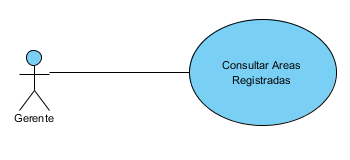
\includegraphics[width=0.8\textwidth]{images/ConsultarAreasRegistradas}
		\caption{Diagrama de Casos de Uso del sistema.}
	\end{figure}